\documentclass[12pt, titlepage]{article}

\usepackage{booktabs}
\usepackage{graphicx}
\usepackage{tabularx}
\usepackage{hyperref}
\usepackage{mdframed}
\hypersetup{
    colorlinks,
    citecolor=black,
    filecolor=black,
    linkcolor=red,
    urlcolor=blue
}
\usepackage[round]{natbib}


\newmdenv[linecolor=black]{reqbox}

\title{SE 3XA3: Requirements Document\\xPyCharts}

\author{Team 4, xPy
		\\ Hatim Rehman (rehmah3)
		\\ Louis Bursey (burseylj)
		\\ Sarthak Desai (desaisa3)
}

\date{\today}

%% Comments

\usepackage{color}

\newif\ifcomments\commentstrue

\ifcomments
\newcommand{\authornote}[3]{\textcolor{#1}{[#3 ---#2]}}
\newcommand{\todo}[1]{\textcolor{red}{[TODO: #1]}}
\else
\newcommand{\authornote}[3]{}
\newcommand{\todo}[1]{}
\fi

\newcommand{\wss}[1]{\authornote{blue}{SS}{#1}}
\newcommand{\ds}[1]{\authornote{red}{DS}{#1}}
\newcommand{\mj}[1]{\authornote{red}{MSN}{#1}}
\newcommand{\cm}[1]{\authornote{red}{CM}{#1}}
\newcommand{\mh}[1]{\authornote{red}{MH}{#1}}

% team members should be added for each team, like the following
% all comments left by the TAs or the instructor should be addressed
% by a corresponding comment from the Team

\newcommand{\tm}[1]{\authornote{magenta}{Team}{#1}}


\begin{document}

\maketitle

\pagenumbering{roman}
\tableofcontents
\listoftables
\listoffigures

\begin{table}[bp]
\caption{\bf Revision History}
\begin{tabularx}{\textwidth}{p{3cm}p{2cm}X}
\toprule {\bf Date} & {\bf Version} & {\bf Notes}\\
\midrule
Oct. 10, 2016 & 1.0 & Revision 0\\
\bottomrule
\end{tabularx}
\end{table}

\newpage

\pagenumbering{arabic}

This document describes the requirements for ....  The template for the Software
Requirements Specification (SRS) is a subset of the Volere
template~\citep{RobertsonAndRobertson2012}.  If you make further modifications
to the template, you should explicity state what modifications were made.

\section{Project Drivers}

\subsection{The Purpose of the Project}

\subsection{The Stakeholders}

\subsubsection{The Client}

\subsubsection{The Customers}

\subsubsection{Other Stakeholders}

\subsection{Mandated Constraints}

\subsection{Naming Conventions and Terminology}

\subsection{Relevant Facts and Assumptions}

User characteristics should go under assumptions.
\clearpage
\section{Functional Requirements}

\subsection{The Scope of the Work and the Product}

\subsubsection{The Context of the Work}
The context can be seen by the following visual, describing user interaction with the program and program response. \\
		
	\begin{figure}[!htb]
		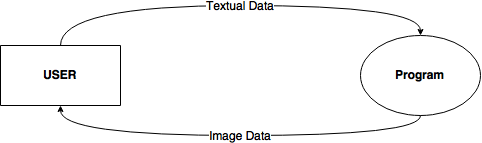
\includegraphics[scale=0.8]{img/ContextDiagram.png}
		\caption{Context Diagram}
	\end{figure}
	
\subsubsection{Work Partitioning}

\begin{center}
\begin{table}[!hpb]
    \caption{Work Partitioning} 
    \begin{tabular}{ |c|p{11cm}|}
	\hline
	Event No. & Event\\ \hline
	1 & Create the (cartesian) coordinate system that is centered within a window.\\ \hline
	2 & Add labels to the coordinate system. \\ \hline
	3 & Plot sample points.\\ \hline
	4 & Construct a line that joins two points together.\\ \hline
	5 & Finishing edits (i.e input checking and error handling).\\ \hline
    \end{tabular}

\end{table}
\end{center}

\subsubsection{Individual Product Use Cases}

Because of the nature of the product, a universal use case exists: 

\begin{reqbox}
    \begin{tabular}{l p{10cm}}

	\bf{Use Case \#: 1} & \\
	 & \\
	{\bfseries Scenario: } 	& 	Constructing a graph from a set of data.	\\
	{\bfseries Trigger: }   		& 	User request. 					\\
	{\bfseries Precondition: } 	&	Data inputted in the correct format.		\\
	{\bfseries PostCondition } 	& 	Graph generated and outputted to the user's screen.				\\

    \end{tabular}
\end{reqbox}


\subsection{Functional Requirements}

\begin{reqbox}
%---
\begin{tabular}{ccc}Requirement \#: 1
\end{tabular} \\
%---
\textbf{Description:} The software shall read data given to it.\\
\textbf{Rationale:} Data is needed to construct a graph. \\
\textbf{Originator:} Hatim Rehman \\
\textbf{Fit Criterion:} The data used by the program is identical to the data given to it.\\
%---
\begin{tabular}{ll}
\textbf{Customer Satisfaction:} 5 & \textbf{Customer Dissatisfaction:} 5 \\
\textbf{Priority:} High & \textbf{Conflicts:} 2,3,4,5\\
\end{tabular} \\
%---  
\textbf{History:} Created October 10, 2016
%--
\end{reqbox}

\begin{reqbox}
%---
\begin{tabular}{ccc}Requirement \#: 2
\end{tabular} \\
%---
\textbf{Description:} The software will raise an exception if the data format cannot be plotted, and stop the program. \\
\textbf{Rationale:} It is safer to stop the program after it is realized the data points do not meet the expected format, versus letting the program proceed to unexpected behaviour. \\
\textbf{Originator:} Hatim Rehman \\
\textbf{Fit Criterion:} The program execution halts when improper data is entered.\\
%---
\begin{tabular}{ll}
\textbf{Customer Satisfaction:} 5 & \textbf{Customer Dissatisfaction:} 5 \\
\textbf{Priority:} High & \textbf{Conflicts:} 3,4,5\\
\end{tabular} \\
%---  
\textbf{History:} Created October 10, 2016
%--
\end{reqbox}

\begin{reqbox}
%---
\begin{tabular}{ccc}Requirement \#: 3
\end{tabular} \\
%---
\textbf{Description:} The software will construct a coordinate system that will fit all the data points.\\
\textbf{Rationale:} This ensures the coordinate system is always dynamically generated to work for all data sets. \\
\textbf{Originator:} Hatim Rehman \\
\textbf{Fit Criterion:} The maximum value on the xy axes is $\geq$ maximum x, y in data set.\\
%---
\begin{tabular}{ll}
\textbf{Customer Satisfaction:} 5 & \textbf{Customer Dissatisfaction:} 5 \\
\textbf{Priority:} High & \textbf{Conflicts:} 4,5\\
\end{tabular} \\
%---  
\textbf{History:} Created October 10, 2016
%--
\end{reqbox}

\begin{reqbox}
%---
\begin{tabular}{ccc}Requirement \#: 4
\end{tabular} \\
%---
\textbf{Description:} The software shall plot all the data points.\\
\textbf{Rationale:} The user will want all the data plotted. \\
\textbf{Originator:} Hatim Rehman \\
\textbf{Fit Criterion:} All data points exist on the generated graph.\\
%---
\begin{tabular}{ll}
\textbf{Customer Satisfaction:} 5 & \textbf{Customer Dissatisfaction:} 5 \\
\textbf{Priority:} High & \textbf{Conflicts:} 5\\
\end{tabular} \\
%---  
\textbf{History:} Created October 10, 2016
%--
\end{reqbox}

\begin{reqbox}
%---
\begin{tabular}{ccc}Requirement \#: 5
\end{tabular} \\
%---
\textbf{Description:} The software will connect a line that passes through all the data points if the data points are a function of x.\\
\textbf{Rationale:} Imposing a constraint on only graphing functions ensures validity and correctness (a function only has one interpretation), whereas graphing relations introduces ambiguity in the shape of the line. \\
\textbf{Originator:} Hatim Rehman \\
\textbf{Fit Criterion:} A line passes through all the points if there is only one y value for each x.\\
%---
\begin{tabular}{ll}
\textbf{Customer Satisfaction:} 5 & \textbf{Customer Dissatisfaction:} 5 \\
\textbf{Priority:} High & \textbf{Conflicts:} None\\
\end{tabular} \\
%---  
\textbf{History:} Created October 10, 2016
%--
\end{reqbox}
\clearpage

\section{Non-functional Requirements} %Louis

\subsection{Look and Feel Requirements}
%
%-----------Visually appealing
%
\begin{reqbox}
%---
\begin{tabular}{ccc}
Requirement \#: 1& Requirement Type: 10a & Event/Use case \#: \\
\end{tabular} \\
%---
\textbf{Description:} The graphs produced should be visually appealing and look professional \\
\textbf{Rationale:} The programmer may be producing graphs for presentations, and will appreciate a good looking product \\
\textbf{Originator:} Louis Bursey\\
\textbf{Fit Criterion:} 70\% of people surveyed believe that graphs are visually appealing and look professional  \\
%---
\begin{tabular}{ll}
\textbf{Customer Satisfaction:} 4 & \textbf{Customer Dissatisfaction:} 2 \\
\textbf{Priority:} Medium & \textbf{Conflicts:} None\\
\end{tabular} \\
%---  
\textbf{Supporting Materials:} None \\
\textbf{History:} Created October 5, 2016
%--
\end{reqbox}
%
% No style req.
%
\subsection{Usability and Humanity Requirements}

%
%-----------Easy to use
%
\begin{reqbox}
%---
\begin{tabular}{ccc}
Requirement \#: & Requirement Type: 11a & Event/Use case \#: \\
\end{tabular} \\
%---
\textbf{Description:} The product should be easy to use for novice Python programmers \\
\textbf{Rationale:} The programmer using this library should be able to focus on their program, not on using this library \\
\textbf{Originator:} Louis Bursey\\
\textbf{Fit Criterion:} 80\% of programmers familiar with Python successfully use the product  \\
%---
\begin{tabular}{ll}
\textbf{Customer Satisfaction:} 4 & \textbf{Customer Dissatisfaction:} 3 \\
\textbf{Priority:} Medium & \textbf{Conflicts:} None\\
\end{tabular} \\
%---  
\textbf{Supporting Materials:} None \\
\textbf{History:} Created October 5, 2016
%--
\end{reqbox}

%
%-----------Language
%
\begin{reqbox}
%---
\begin{tabular}{ccc}
Requirement \#: & Requirement Type: 11b & Event/Use case \#: \\
\end{tabular} \\
%---
\textbf{Description:} When natural language is required, this product will use English \\
\textbf{Rationale:} Python is written in English \\
\textbf{Originator:} Louis Bursey\\
\textbf{Fit Criterion:}  No non-English natural language is used in the product \\
%---
\begin{tabular}{ll}
\textbf{Customer Satisfaction:} 1 & \textbf{Customer Dissatisfaction:} 5 \\
\textbf{Priority:} High & \textbf{Conflicts:} None\\
\end{tabular} \\
%---  
\textbf{Supporting Materials:} None \\
\textbf{History:} Created October 5, 2016
%--
\end{reqbox}
%
% No personalization unless you mean the actual graphs, I believe that would be a functional requirement?
%
%
%-----------Quick to learn
%
\begin{reqbox}
%---
\begin{tabular}{ccc}
Requirement \#: & Requirement Type: 11c & Event/Use case \#: \\
\end{tabular} \\
%---
\textbf{Description:} The programmer using this product should quickly be able to learn how to use this product \\
\textbf{Rationale:} Programmers who face a steep learning curve will be discouraged from using this product \\
\textbf{Originator:} Louis Bursey\\
\textbf{Fit Criterion:}  Programmers familiar with Python are able to produce graphs within an average twenty minutes of acquiring the library \\
%---
\begin{tabular}{ll}
\textbf{Customer Satisfaction:} 4 & \textbf{Customer Dissatisfaction:} 4 \\
\textbf{Priority:} Medium & \textbf{Conflicts:} None\\
\end{tabular} \\
%---  
\textbf{Supporting Materials:} None \\
\textbf{History:} Created October 5, 2016
\end{reqbox}
%
%-----------Error messages
%
\begin{reqbox}
%---
\begin{tabular}{ccc}
Requirement \#: & Requirement Type: 11d & Event/Use case \#: \\
\end{tabular} \\
%---
\textbf{Description:} When used incorrectly, the product should generate error messages that are easy to understand \\
\textbf{Rationale:} Knowing when and how the library is being used incorrectly will help developers use the library more efficiently. \\
\textbf{Originator:} Louis Bursey\\
\textbf{Fit Criterion:}  80\% of programmers using the library for the first time can understand the error messages they create \\
%---
\begin{tabular}{ll}
\textbf{Customer Satisfaction:} 5 & \textbf{Customer Dissatisfaction:} 4 \\
\textbf{Priority:} High & \textbf{Conflicts:} None\\
\end{tabular} \\
%---  
\textbf{Supporting Materials:} None \\
\textbf{History:} Created October 5, 2016
%--
\end{reqbox}
%
% No accessibility, outside of the scope of this project
%

\subsection{Performance Requirements}
%
%-----------Speed
%
\begin{reqbox}
%---
\begin{tabular}{ccc}
Requirement \#: & Requirement Type: 12a & Event/Use case \#: \\
\end{tabular} \\
%---
\textbf{Description:} The product should generate graphs in a timely manner \\
\textbf{Rationale:} The program should not take so long that it slows down the programmer's workflow \\
\textbf{Originator:} Louis Bursey\\
\textbf{Fit Criterion:}  The library takes under 20 seconds to generate graphs of a reasonable size \\
%---
\begin{tabular}{ll}
\textbf{Customer Satisfaction:} 4 & \textbf{Customer Dissatisfaction:} 4 \\
\textbf{Priority:} High & \textbf{Conflicts:} None\\
\end{tabular} \\
%---  
\textbf{Supporting Materials:} None \\
\textbf{History:} Created October 5, 2016
%--
\end{reqbox}
%
% No safety critical requirements
%

%
%-----------Precision                                                     %confirm on precision
%
\begin{reqbox}
%---
\begin{tabular}{ccc}
Requirement \#: & Requirement Type: 12c & Event/Use case \#: \\
\end{tabular} \\
%---
\textbf{Description:} The product should produce accurate graphs \\
\textbf{Rationale:} Visual representations of data are useless if they don't represent data faithfully \\
\textbf{Originator:} Louis Bursey\\
\textbf{Fit Criterion:}  Graphs produced should have no less than 20\% difference between it and a graph generated by JCharts  \\
%---
\begin{tabular}{ll}
\textbf{Customer Satisfaction:} 5 & \textbf{Customer Dissatisfaction:} 5 \\
\textbf{Priority:} High & \textbf{Conflicts:} None\\
\end{tabular} \\
%---  
\textbf{Supporting Materials:} None \\
\textbf{History:} Created October 5, 2016
%--
\end{reqbox}
%
%-----------Reliability
%
\begin{reqbox}
%---
\begin{tabular}{ccc}
Requirement \#: & Requirement Type: 12d & Event/Use case \#: \\
\end{tabular} \\
%---
\textbf{Description:} The product should always be available \\
\textbf{Rationale:} The product cannot unexpectedly go out of service, as programmers will depend on its availability \\
\textbf{Originator:} Louis Bursey\\
\textbf{Fit Criterion:}  The product is always available  \\
%---
\begin{tabular}{ll}
\textbf{Customer Satisfaction:} 1 & \textbf{Customer Dissatisfaction:} 5 \\
\textbf{Priority:} High & \textbf{Conflicts:} None\\
\end{tabular} \\
%---  
\textbf{Supporting Materials:} None \\
\textbf{History:} Created October 5, 2016
%--
\end{reqbox}
%
%-----------Robustness
%
\begin{reqbox}
%---
\begin{tabular}{ccc}
Requirement \#: & Requirement Type: 12e & Event/Use case \#: \\
\end{tabular} \\
%---
\textbf{Description:} The library will not stall out, if used incorrectly it will always display error messages and abort\\
\textbf{Rationale:} Programmers using the library will depend on graphs not stalling out their programs \\
\textbf{Originator:} Louis Bursey\\
\textbf{Fit Criterion:}    Errors in use always create error messages and aborts, not stalls\\
%---
\begin{tabular}{ll}
\textbf{Customer Satisfaction:} 1 & \textbf{Customer Dissatisfaction:} 5 \\
\textbf{Priority:} High & \textbf{Conflicts:} None\\
\end{tabular} \\
%---  
\textbf{Supporting Materials:} None \\
\textbf{History:} Created October 5, 2016
%--
\end{reqbox}
%
%-----------Capacity                     %%%confirm on graph size
%
\begin{reqbox}
%---
\begin{tabular}{ccc}
Requirement \#: & Requirement Type: 12f & Event/Use case \#: \\
\end{tabular} \\
%---
\textbf{Description:} The library will be able to produce graphs with up to 500 data points \\
\textbf{Rationale:} Programmers using the library will want to build graphs from large data sets \\
\textbf{Originator:} Louis Bursey\\
\textbf{Fit Criterion:}  Graph with up to 500 data points can be generated without problems\\
%---
\begin{tabular}{ll}
\textbf{Customer Satisfaction:} 3 & \textbf{Customer Dissatisfaction:} 5 \\
\textbf{Priority:} High & \textbf{Conflicts:} None\\
\end{tabular} \\
%---  
\textbf{Supporting Materials:} None \\
\textbf{History:} Created October 5, 2016
%--
\end{reqbox}
%
% No scalability
%
% No longevity
%
\subsection{Operational and Environmental Requirements}

%
%-----------Environment---PCs                 
%
\begin{reqbox}
%---
\begin{tabular}{ccc}
Requirement \#: & Requirement Type: 13a & Event/Use case \#: \\
\end{tabular} \\
%---
\textbf{Description:} The product should operate on laptops and desktops \\
\textbf{Rationale:} Programmers work on laptops and desktops and the library should work in this environment \\
\textbf{Originator:} Louis Bursey\\
\textbf{Fit Criterion:}  Personal computer users can run programs that use the library\\
%---
\begin{tabular}{ll}
\textbf{Customer Satisfaction:} 3 & \textbf{Customer Dissatisfaction:} 5 \\
\textbf{Priority:} High & \textbf{Conflicts:} None\\
\end{tabular} \\
%---  
\textbf{Supporting Materials:} None \\
\textbf{History:} Created October 5, 2016
%--
\end{reqbox}

%
%-----------Environment---Python                     
%
\begin{reqbox}
%---
\begin{tabular}{ccc}
Requirement \#: & Requirement Type: 13a & Event/Use case \#: \\
\end{tabular} \\
%---
\textbf{Description:} The product should be usable as a Pyton library \\
\textbf{Rationale:} The Python language is the supported language of this project\\
\textbf{Originator:} Louis Bursey\\
\textbf{Fit Criterion:}  The product is importable in a Python program\\
%---
\begin{tabular}{ll}
\textbf{Customer Satisfaction:} 1 & \textbf{Customer Dissatisfaction:} 5 \\
\textbf{Priority:} High & \textbf{Conflicts:} None\\
\end{tabular} \\
%---  
\textbf{Supporting Materials:} None \\
\textbf{History:} Created October 5, 2016
%--
\end{reqbox}
%
%
% Don't think it needs to interface, confirm?
%
%
%-----------Productization
%
\begin{reqbox}
%---
\begin{tabular}{ccc}
Requirement \#: & Requirement Type: 13c & Event/Use case \#: \\
\end{tabular} \\
%---
\textbf{Description:} \\
\textbf{Rationale:} The product should be distributed as a zip file that is importable in Python programs\\
\textbf{Originator:} Louis Bursey\\
\textbf{Fit Criterion:}  The product is importable in a Python program\\
%---
\begin{tabular}{ll}
\textbf{Customer Satisfaction:} 3 & \textbf{Customer Dissatisfaction:} 4 \\
\textbf{Priority:} High & \textbf{Conflicts:} None\\
\end{tabular} \\
%---  
\textbf{Supporting Materials:} None \\
\textbf{History:} Created October 5, 2016
%--
\end{reqbox}

%
%-----------Release
%
\begin{reqbox}
%---
\begin{tabular}{ccc}
Requirement \#: & Requirement Type: 13d & Event/Use case \#: \\
\end{tabular} \\
%---
\textbf{Description:}Future releases of the project will be backwards compatible \\
\textbf{Rationale:} Backwards compatibility keeps programmers from having to update their code when we make changes\\
\textbf{Originator:} Louis Bursey\\
\textbf{Fit Criterion:}  Releases are backwards compatible\\
%---
\begin{tabular}{ll}
\textbf{Customer Satisfaction:} 2 & \textbf{Customer Dissatisfaction:} 5 \\
\textbf{Priority:} High & \textbf{Conflicts:} None\\
\end{tabular} \\
%---  
\textbf{Supporting Materials:} None \\
\textbf{History:} Created October 5, 2016
%--
\end{reqbox}

\subsection{Maintainability and Support Requirements}
%
% no maintenance requirements for this project
%
% No support requirements for this project
%
%
%-----------Adaptability to OS's
%
\begin{reqbox}
%---
\begin{tabular}{ccc}
Requirement \#: & Requirement Type: 13d & Event/Use case \#: \\
\end{tabular} \\
%---
\textbf{Description:}The product should work in Windows, Linux and Mac OSX environments \\
\textbf{Rationale:} Programmers working in all of these environments will need graphing capabilities\\
\textbf{Originator:} Louis Bursey\\
\textbf{Fit Criterion:}  The library is usable in all of these environments \\
%---
\begin{tabular}{ll}
\textbf{Customer Satisfaction:} 4 & \textbf{Customer Dissatisfaction:} 5 \\
\textbf{Priority:} High & \textbf{Conflicts:} None\\
\end{tabular} \\
%---  
\textbf{Supporting Materials:} None \\
\textbf{History:} Created October 5, 2016
%--
\end{reqbox}


\subsection{Security Requirements}
There are no security requirements for this project
\subsection{Cultural Requirements}
There are no cultural requirements for this project
\subsection{Legal Requirements}
There are no legal requirements for this project
\subsection{Health and Safety Requirements} %end Louis

A graphing library does not pose any serious health and safety risks.

\clearpage
\section{Project Issues}

\subsection{Open Issues}

\subsection{Off-the-Shelf Solutions}

\subsection{New Problems}

\subsection{Tasks} 

\subsection{Migration to the New Product}

\subsection{Risks}

\subsection{Costs}

\subsection{User Documentation and Training}

\subsection{Waiting Room}

\subsection{Ideas for Solutions}

\bibliographystyle{plainnat}

\bibliography{SRS}

\newpage

\section{Appendix}

This section has been added to the Volere template.  This is where you can place
additional information.

\subsection{Symbolic Parameters}

The definition of the requirements will likely call for SYMBOLIC\_CONSTANTS.
Their values are defined in this section for easy maintenance.

\subsection{Gantt Chart}

The schedule of the project is shown by the following
 \href{run:../DevelopmentPlan/GanttChart.gan} {\underline{Gantt Chart}}.

\end{document}